\documentclass[12pt,letterpaper]{article}
\usepackage{graphicx,textcomp}
\usepackage{natbib}
\usepackage{setspace}
\usepackage{fullpage}
\usepackage{color}
\usepackage[reqno]{amsmath}
\usepackage{amsthm}
\usepackage{fancyvrb}
\usepackage{amssymb,enumerate}
\usepackage[all]{xy}
\usepackage{endnotes}
\usepackage{lscape}
\newtheorem{com}{Comment}
\usepackage{float}
\usepackage{hyperref}
\newtheorem{lem} {Lemma}
\newtheorem{prop}{Proposition}
\newtheorem{thm}{Theorem}
\newtheorem{defn}{Definition}
\newtheorem{cor}{Corollary}
\newtheorem{obs}{Observation}
\usepackage[compact]{titlesec}
\usepackage{dcolumn}
\usepackage{tikz}
\usetikzlibrary{arrows}
\usepackage{multirow}
\usepackage{xcolor}
\newcolumntype{.}{D{.}{.}{-1}}
\newcolumntype{d}[1]{D{.}{.}{#1}}
\definecolor{light-gray}{gray}{0.65}
\usepackage{url}
\usepackage{listings}
\usepackage{color}

\definecolor{codegreen}{rgb}{0,0.6,0}
\definecolor{codegray}{rgb}{0.5,0.5,0.5}
\definecolor{codepurple}{rgb}{0.58,0,0.82}
\definecolor{backcolour}{rgb}{0.95,0.95,0.92}

\lstdefinestyle{mystyle}{
	backgroundcolor=\color{backcolour},   
	commentstyle=\color{codegreen},
	keywordstyle=\color{magenta},
	numberstyle=\tiny\color{codegray},
	stringstyle=\color{codepurple},
	basicstyle=\footnotesize,
	breakatwhitespace=false,         
	breaklines=true,                 
	captionpos=b,                    
	keepspaces=true,                 
	numbers=left,                    
	numbersep=5pt,                  
	showspaces=false,                
	showstringspaces=false,
	showtabs=false,                  
	tabsize=2
}
\lstset{style=mystyle}
\newcommand{\Sref}[1]{Section~\ref{#1}}
\newtheorem{hyp}{Hypothesis}

\title{Problem Set 2}
\date{Due: October 22, 2026}
\author{Applied Stats/Quant Methods 1}

\begin{document}
	\maketitle
	\section*{Instructions}
\begin{itemize}
	\item Please show your work! You may lose points by simply writing in the answer. If the problem requires you to execute commands in \texttt{R}, please include the code you used to get your answers. Please also include the \texttt{.R} file that contains your code. If you are not sure if work needs to be shown for a particular problem, please ask.
	\item Your homework should be submitted electronically on GitHub.
	\item This problem set is due before 23:59 on Thursday October 22, 2026. No late assignments will be accepted.

\end{itemize}

	
	\vspace{.5cm}
	\section*{Question 1: Political Science}
		\vspace{.25cm}
	The following table was created using the data from a study run in a major Latin American city.\footnote{Fried, Lagunes, and Venkataramani (2010). ``Corruption and Inequality at the Crossroad: A Multimethod Study of Bribery and Discrimination in Latin America. \textit{Latin American Research Review}. 45 (1): 76-97.} As part of the experimental treatment in the study, one employee of the research team was chosen to make illegal left turns across traffic to draw the attention of the police officers on shift. Two employee drivers were upper class, two were lower class drivers, and the identity of the driver was randomly assigned per encounter. The researchers were interested in whether officers were more or less likely to solicit a bribe from drivers depending on their class (officers use phrases like, ``We can solve this the easy way'' to draw a bribe). The table below shows the resulting data.

\newpage
\begin{table}[h!]
	\centering
	\begin{tabular}{l | c c c }
		& Not Stopped & Bribe requested & Stopped/given warning \\
		\\[-1.8ex] 
		\hline \\[-1.8ex]
		Upper class & 14 & 6 & 7 \\
		Lower class & 7 & 7 & 1 \\
		\hline
	\end{tabular}
\end{table}

\begin{enumerate}
	
	\item [(a)]
	Calculate the $\chi^2$ test statistic by hand/manually (even better if you can do "by hand" in \texttt{R}).\\
	
	
	As we have two categorical variables, we use the $chi-test$ for \textbf{statistical independence}. The test statistic is calculated with the following formula:  $$\chi^2 = \sum_{i=1}^{k} \frac{(f_{o} - f_{e})^2}{f_{e}}$$
	
	Where $f_{e,i}$ is calculated with the formula:
	
	\begin{equation}
		f_{e} = \frac{\text{Row Total} \cdot \text{Column Total}}{\text{Total Observations}}
	\end{equation}
	
	I did it partly manually in R, using matrices and the way R handles mathematical operations with this data structure. First, I created a matrix containing the values of our contingency table. 
	
	\lstinputlisting[firstline = 36, lastline = 36]{PS02_AL.R}
	
	By combining indexing with R's sum() function, we can now calculate the expected value for each cell. Since there are only 6 cells, I write out the formula explicitly.  
	
	\begin{verbatim}
> expected_frequency <- matrix(c(
+   sum(experiment[1, ]) * sum(experiment[, 1])/sum(experiment),
+   sum(experiment[1, ]) * sum(experiment[, 2])/sum(experiment),
+   sum(experiment[1, ]) * sum(experiment[, 3])/sum(experiment),
+   sum(experiment[2, ]) * sum(experiment[, 1])/sum(experiment),
+   sum(experiment[2, ]) * sum(experiment[, 2])/sum(experiment),
+   sum(experiment[2, ]) * sum(experiment[, 3])/sum(experiment)
+ ), nrow = 2, byrow = TRUE)
> expected_frequency
[,1]     [,2]     [,3]
[1,] 13.5 8.357143 5.142857
[2,]  7.5 4.642857 2.857143
	\end{verbatim}

Next, I calculated the $\chi^2$ for each cell and summed them. I did this for two reasons: first, I discussed the problem set results with fellow students, which let us compare them more easily. Second, I thought this might help calculate the standardized residuals. However, I ended up using the full formula for the standardized residuals because I wanted to make sure that my probability calculations for rows and columns worked correctly.

	\begin{verbatim}
		    [,1]     [,2]     [,3]
		[1,] 13.5 8.357143 5.142857
		[2,]  7.5 4.642857 2.857143
		> chi_squared <- (experiment - expected_frequency)**2 / expected_frequency
		> chi_squared 
		[,1]      [,2]      [,3]
		[1,] 0.01851852 0.6648352 0.6706349
		[2,] 0.03333333 1.1967033 1.2071429
		> sum(chi_squared) # Chi-squared has a value of 3.791168
		[1] 3.791168
		> chi_sum <- sum(chi_squared)
		> chi_sum
		[1] 3.791168
	\end{verbatim}
	
		
	\item [(b)]
	Now calculate the p-value from the test statistic you just created (in \texttt{R}).\footnote{Remember frequency should be $>$ 5 for all cells, but let's calculate the p-value here anyway.}  What do you conclude if $\alpha = 0.1$?\\
	
	
	Using the \texttt{chi\_sum} object from the previous task, I used the approriate R function:
	
	\lstinputlisting[firstline = 55, lastline = 57]{PS02_AL.R}
	
	The probability of a $\chi^2$ value that is as large as our empirical $\chi^2$ or larger is 0.1502. Therefore, we cannot reject H0 at an alpha level of 0.1, as $0.1502 > 0.10$. Based on our test the variables are \textbf{statistically independent}.
	
	
	\newpage
	\item [(c)] Calculate the standardized residuals for each cell and put them in the table below.
	\vspace{1cm}
	
	I again used my matrix object to calculate the row and column probabilities. Afterward, I used cbind and rbind to create matrices that contain the values in a format to calculate with, without running into problems based on R’s recycling of shorter vectors.
	
	\begin{verbatim}
		> p_row = rowSums(experiment) / sum(experiment)
		> p_column = colSums(experiment) / sum(experiment)
		> 
		> p_row_matrix <- cbind(p_row, p_row, p_row)
		> p_column_matrix <- rbind(p_column, p_column)
		> p_row_matrix
		p_row     p_row     p_row
		[1,] 0.6428571 0.6428571 0.6428571
		[2,] 0.3571429 0.3571429 0.3571429
		> p_column_matrix 
		[,1]      [,2]      [,3]
		p_column  0.5 0.3095238 0.1904762
		p_column  0.5 0.3095238 0.1904762
	\end{verbatim}
	
	I plugged this matrices in the formula and received:
	
	\begin{verbatim}
		> pearson_res <- (experiment - expected_frequency) / sqrt(expected_frequency * (1 - p_row_matrix) * (1 - p_column_matrix))
		> pearson_res
		p_row     p_row     p_row
		[1,]  0.3220306 -1.641957  1.523026
		[2,] -0.3220306  1.641957 -1.523026
		
	\end{verbatim}
	
	The results could be used to fill the table. 
	
	\begin{table}[h]
		\centering
		\begin{tabular}{l | c c c }
			& Not Stopped & Bribe requested & Stopped/given warning \\
			\\[-1.8ex] 
			\hline \\[-1.8ex]
			Upper class & 0.3220306 & -1.641957 & 1.523026  \\
			\\
			Lower class & -0.3220306 & 1.641957 & -1.523026   \\
			
		\end{tabular}
	\end{table}
	
	
	\vspace{7cm}
	\item [(d)] How might the standardized residuals help you interpret the results?  
	
	Generally, the \textit{not-stopped} category is very close to the expected value, while the \textit{bribe accepted”} and \textit{warned} categories show somewhat larger adjusted residuals. 
	\newline
	This may indicate that our experimental treatment did not affect whether someone was stopped in the first place, but rather whether the police officer accepted a bribe after they stopped someone. One confounding reason could be that police officers decided to stop cars based on factors outside our experimental treatment (e.g., a desire to make a break). Therefore, it may be reasonable to recalculate the test statistic without the not-stopped category. 
	
	
\end{enumerate}
\newpage

\section*{Question 2: Economics}
Chattopadhyay and Duflo were interested in whether women promote different policies than men.\footnote{Chattopadhyay and Duflo. (2004). ``Women as Policy Makers: Evidence from a Randomized Policy Experiment in India. \textit{Econometrica}. 72 (5), 1409-1443.} Answering this question with observational data is pretty difficult due to potential confounding problems (e.g. the districts that choose female politicians are likely to systematically differ in other aspects too). Hence, they exploit a randomized policy experiment in India, where since the mid-1990s, $\frac{1}{3}$ of village council heads have been randomly reserved for women. A subset of the data from West Bengal can be found at the following link: \url{https://raw.githubusercontent.com/kosukeimai/qss/master/PREDICTION/women.csv}\\

\lstinputlisting[firstline = 96, lastline = 96]{PS02_AL.R}

\noindent Each observation in the data set represents a village and there are two villages associated with one GP (i.e. a level of government is called "GP"). Figure~\ref{fig:women_desc} below shows the names and descriptions of the variables in the dataset. The authors hypothesize that female politicians are more likely to support policies female voters want. Researchers found that more women complain about the quality of drinking water than men. You need to estimate the effect of the reservation policy on the number of new or repaired drinking water facilities in the villages.
\vspace{.5cm}
\begin{figure}[h!]
	\caption{\footnotesize{Names and description of variables from Chattopadhyay and Duflo (2004).}}
	\vspace{.5cm}
	\centering
	\label{fig:women_desc}
	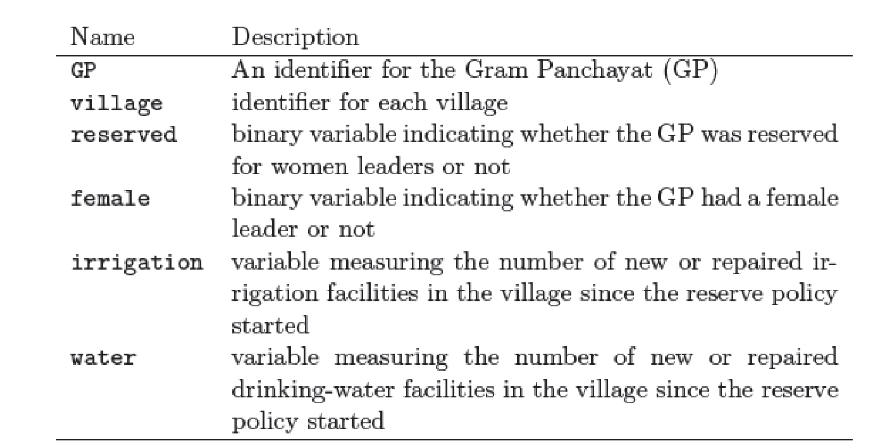
\includegraphics[width=0.8\textwidth]{Figure1}
\end{figure}		


\newpage
\begin{enumerate}
	\item [(a)] State a null and alternative (two-tailed) hypothesis. 
	
	\begin{center}
		\textbf{$H_0$:} The number of water facilities is not different between villages with reserved seats at the GP level and villages without reserved seats at the GP level.\\[1em]
		\textbf{$H_1$:} The number of water facilities is different between villages with reserved seats at the GP level and villages without reserved seats at the GP level.
	\end{center}
	
	
	\vspace{6cm}
	\item [(b)] Run a bivariate regression to test this hypothesis in \texttt{R} (include your code!).
	
	\begin{verbatim}
		> model_india <- lm(data = df_india,
		+                   water ~ as.factor(reserved))
		> summary(model_india)
		
		Call:
		lm(formula = water ~ as.factor(reserved), data = df_india)
		
		Residuals:
		Min      1Q  Median      3Q     Max 
		-23.991 -14.738  -7.865   2.262 316.009 
		
		Coefficients:
		Estimate Std. Error t value Pr(>|t|)    
		(Intercept)            14.738      2.286   6.446 4.22e-10 ***
		as.factor(reserved)1    9.252      3.948   2.344   0.0197 *  
		---
		Signif. codes:  0 ‘***’ 0.001 ‘**’ 0.01 ‘*’ 0.05 ‘.’ 0.1 ‘ ’ 1
		
		Residual standard error: 33.45 on 320 degrees of freedom
		Multiple R-squared:  0.01688,	Adjusted R-squared:  0.0138 
		F-statistic: 5.493 on 1 and 320 DF,  p-value: 0.0197
	\end{verbatim}
	
	The p-value of $0.0197 < 0.05$. Therefore, we can reject the $H0$. In other words, there is a difference in repaired or newly installed water facilities between villages with and without a reservation policy at the gp level.
	However, we should be aware that the observations are not really independent, as villages from the same GP will very likely deviate from our estimate in the same way.
	
	\item [(c)] Interpret the coefficient estimate for reservation policy. 
	
	Without a categorical (binary) covariate, the intercept estimates the value for the reference category ($reservation policy = 0$), while the slope captures the difference between villages with and without a reservation policy.
	Specifically, villages in GPs without a reservation policy saw $14.73$ facilities repaired or newly installed, while villages with a reservation policy saw an additional $9.25$ facilities repaired or newly installed, for a total of about 24 repaired or newly installed facilities.
	
	
\end{enumerate}


%\end{enumerate}
\end{document}
